\documentclass[11pt]{article}
\usepackage[utf8]{inputenc}
\usepackage{amsfonts}
\usepackage{natbib}
\usepackage{graphicx}
\usepackage{amsmath}
\usepackage{amssymb}
\usepackage{mathrsfs} % Cursive font
\usepackage{graphicx}
\usepackage{ragged2e}
\usepackage{fancyhdr}
\usepackage{nameref}
\usepackage{wrapfig}
\usepackage{hyperref}


\usepackage{mathtools}
\usepackage{xparse} \DeclarePairedDelimiterX{\Iintv}[1]{\llbracket}{\rrbracket}{\iintvargs{#1}}
\NewDocumentCommand{\iintvargs}{>{\SplitArgument{1}{,}}m}
{\iintvargsaux#1}
\NewDocumentCommand{\iintvargsaux}{mm} {#1\mkern1.5mu,\mkern1.5mu#2}

\makeatletter
\newcommand*{\currentname}{\@currentlabelname}
\makeatother



\addtolength{\textwidth}{0.2cm}
\setlength{\parskip}{8pt}
\setlength{\parindent}{0.5cm}
\linespread{1.5}

\pagestyle{fancy}
\fancyhf{}
\rhead{TP2 - Cipullo}
\lhead{Seguridad Informática}
\rfoot{\vspace{1cm} \thepage}

\renewcommand*\contentsname{\LARGE Índice}

\setlength{\skip\footins}{0.5cm}

\begin{document}

\begin{titlepage}
    \hspace{-2.5cm}
\includegraphics[scale= 0.48]{../header.png}
    \begin{center}
        \vfill
            \noindent\textbf{\Huge Seguridad Informática}\par
            \vspace{.5cm}
            \noindent\textbf{\Huge Trabajo Práctico 2}\par
            \vspace{.5cm}
        \vfill
        \noindent \textbf{\huge Alumna:}\par
        \vspace{.5cm}
        \noindent \textbf{\Large Cipullo, Inés}\par
 
        \vfill
        % \large Universidad Nacional de Rosario \par
        \noindent\large 2023
    \end{center}
\end{titlepage}
\ \par

\section*{SQL Inyection}
Tema realizado en modo avanzado.

\subsection*{Task 1}
Luego de abrir la consola de \verb|mysql| y cargar la base de datos ya existente en la VM, \verb|Users|, 
corro el comando \verb|mysql> show tables;| para mostrar las tablas de la base de datos. Vemos que hay 
una única tabla, \verb|credential|, que se entiende que contiene la información de los perfiles del sistema.
Con el comando \verb|mysql> select * from credentail;|, se imprimen todas las filas y columnas de la tabla,
el output del comando fue el siguiente:

\begin{center}
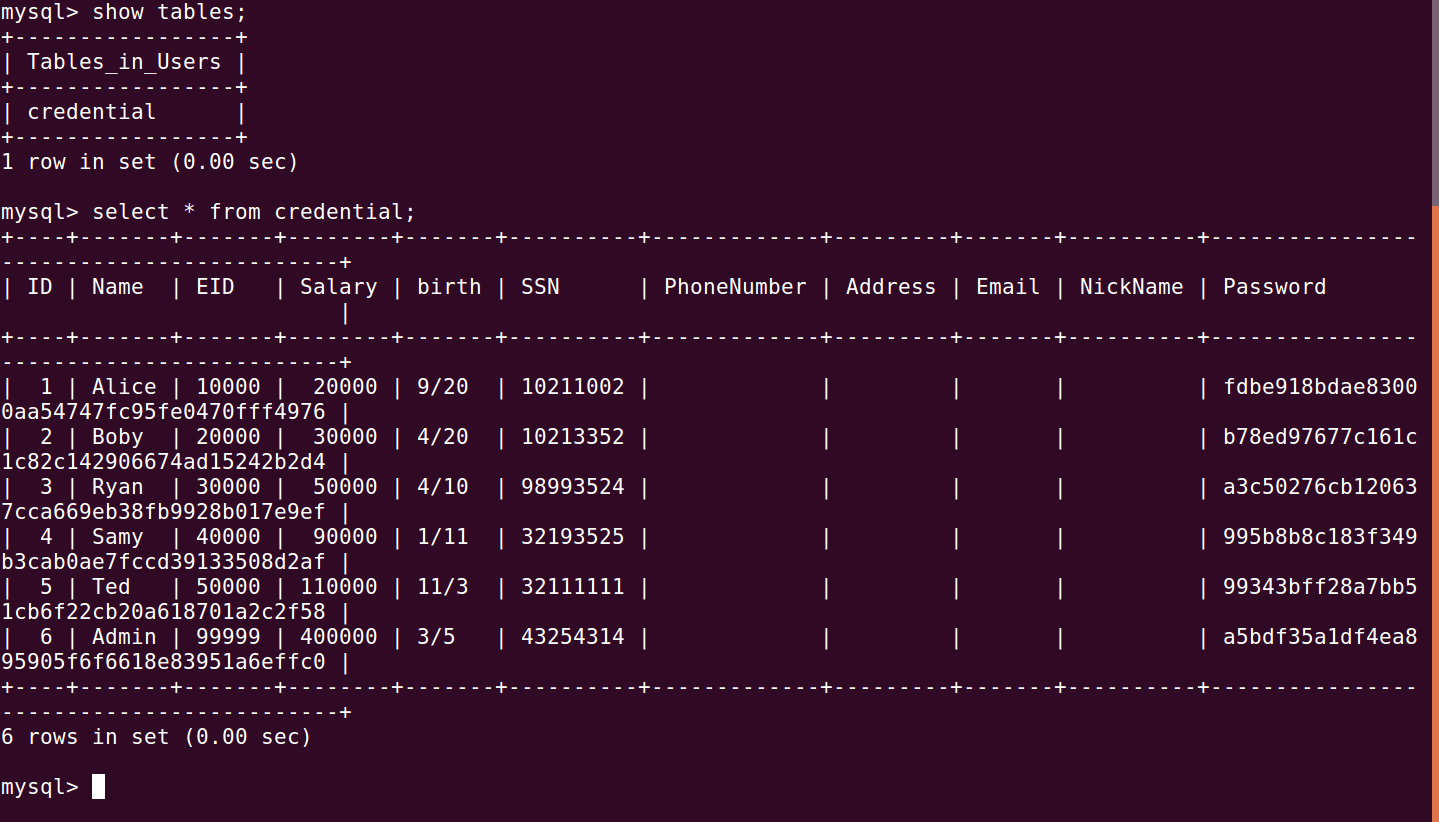
\includegraphics[scale=.34]{task1_sql.png}
\end{center}

Una vez que se conocen la estructura y el contenido de la tabla, para obtener solo la información de pérfil
de \textit{Alice}, se puede correr el siguiente comando: \verb|select * from credential where Name = 'Alice';|.

\subsection*{Task 2}

\subsubsection*{Task 2.1}
La idea es autenticarse en la página web como administrador para poder tener acceso a los datos de todos los 
perfiles, pero sabiendo unicamente que el usuario es \verb|admin|, sin conocer la contraseña.

Luego de entender cómo está implementada la autenticación de la página web, nos damos cuenta que no se utilizan 
queries parametrizadas, sino que el usuario y contraseña que se ingresan son agregados a la query como texto plano.
Analizando la estructura de la query, vemos que ingresando el usuario del administrador y comentando el resto de la
query, se puede lograr autenticarse como administrador.

Como usuario entonces utilizamos \verb|admin'#|, la comilla para indicar que finaliza el nombre que se quiere 
ingresar y el numeral para comentar el resto de la query. Esto significa que en la contraseña no hace falta poner
nada porque no se la utiliza para la query y aparte no hay validación de los datos que se ingresan.

Desde la página de login, entonces, ingresamos de la siguiente manera:
\begin{center}
    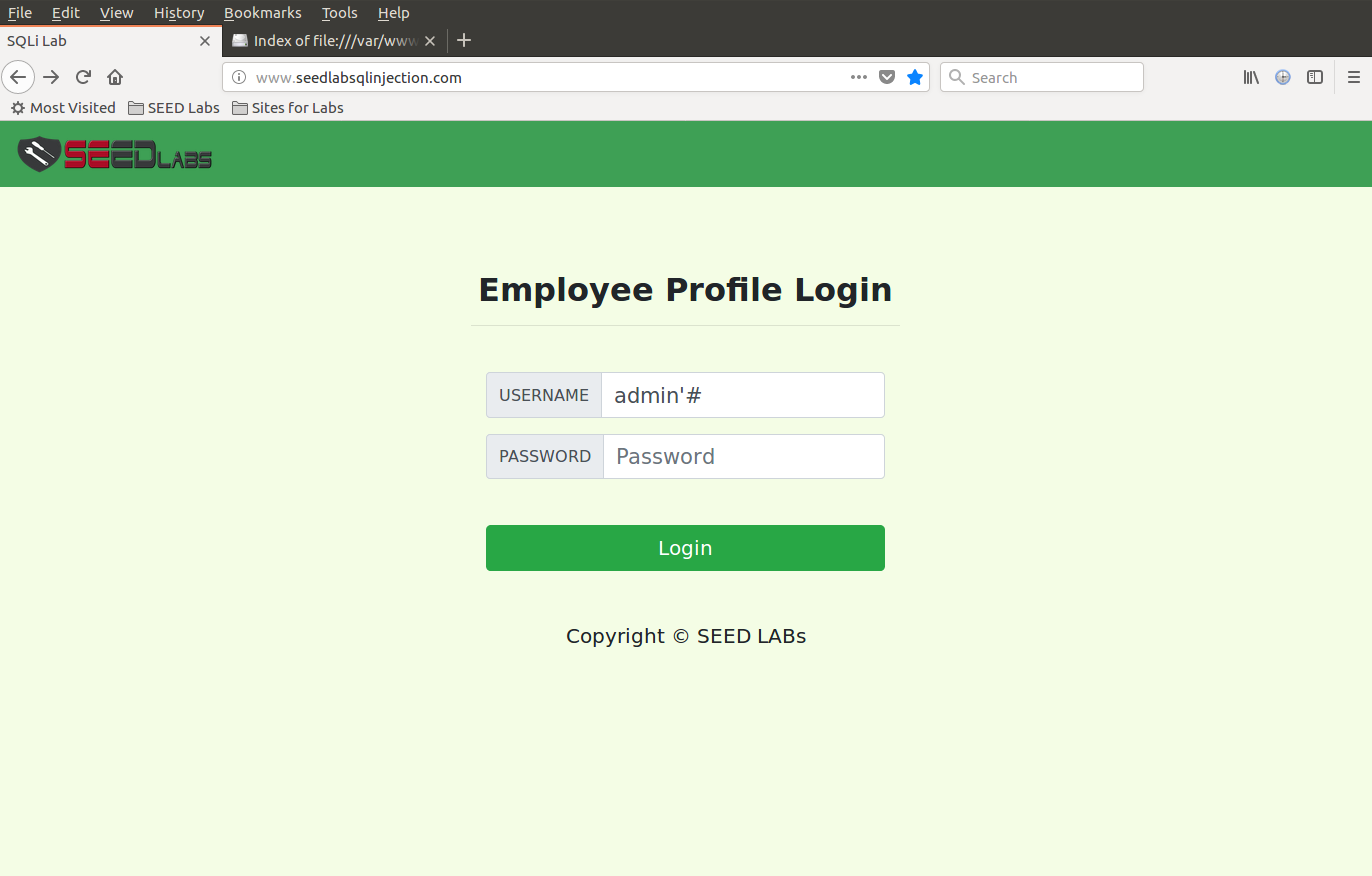
\includegraphics[scale=.34]{task2_1_1_sql.png}
\end{center}

Luego de apretar el botón de \verb|Login|, obtenemos la información de todos los perfiles:
\begin{center}
    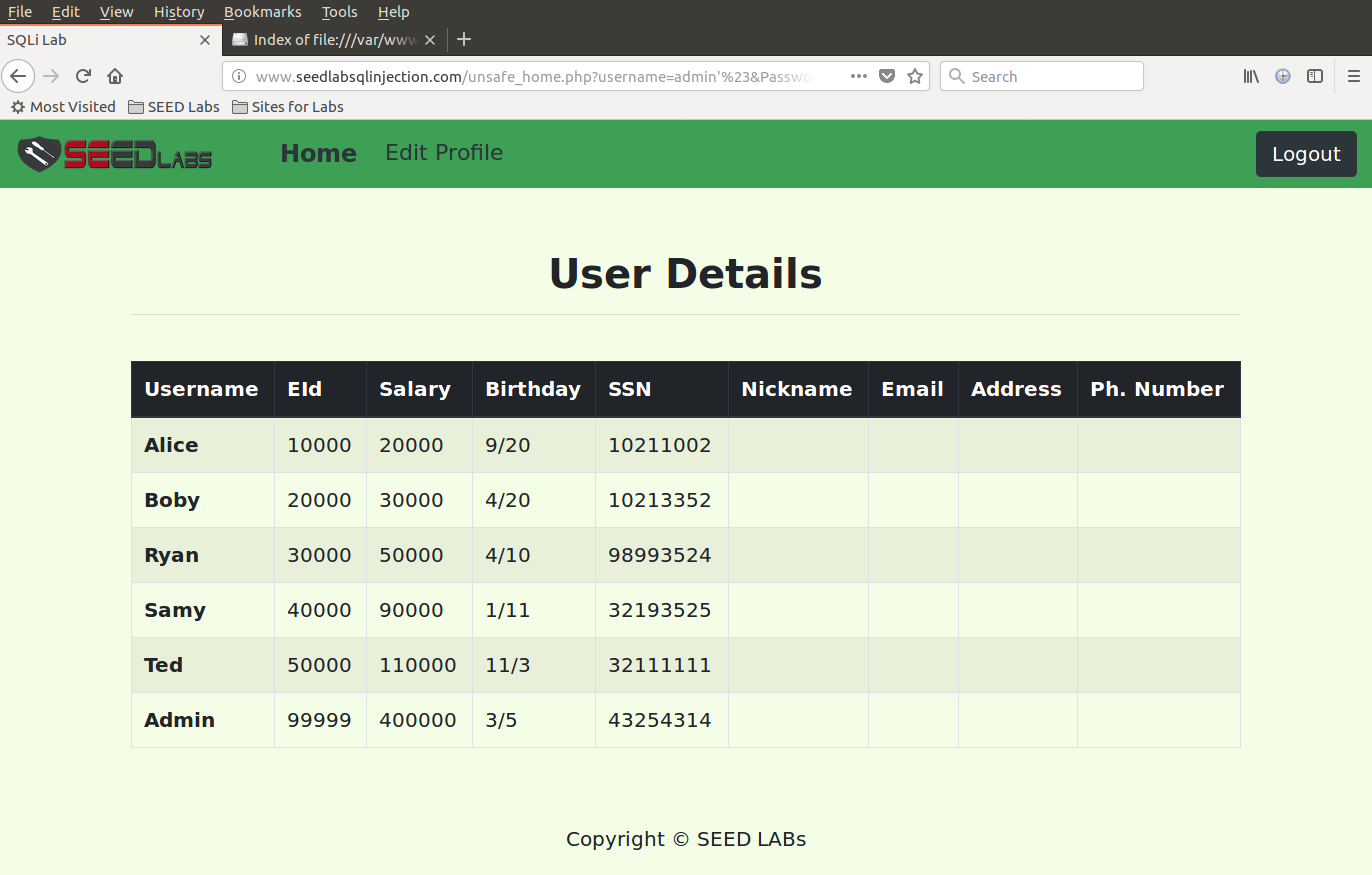
\includegraphics[scale=.34]{task2_1_2_sql.png}
\end{center}

\subsubsection*{Task 2.2}
Ahora, buscamos repetir el ataque del punto anterior pero enviando solicitudes HTTP a travéz de líneas de comando
y no utilizando la página web.

Para lograrlo, utilizamos \verb|curl| y le pasamos la URL de la página incluyendo los parámetrocs de usuario 
y contraseña. Efectivamente obtenemos como respuesta el HTML donde se muesta la información de todos los usuarios.
Como sigue:
\begin{center}
    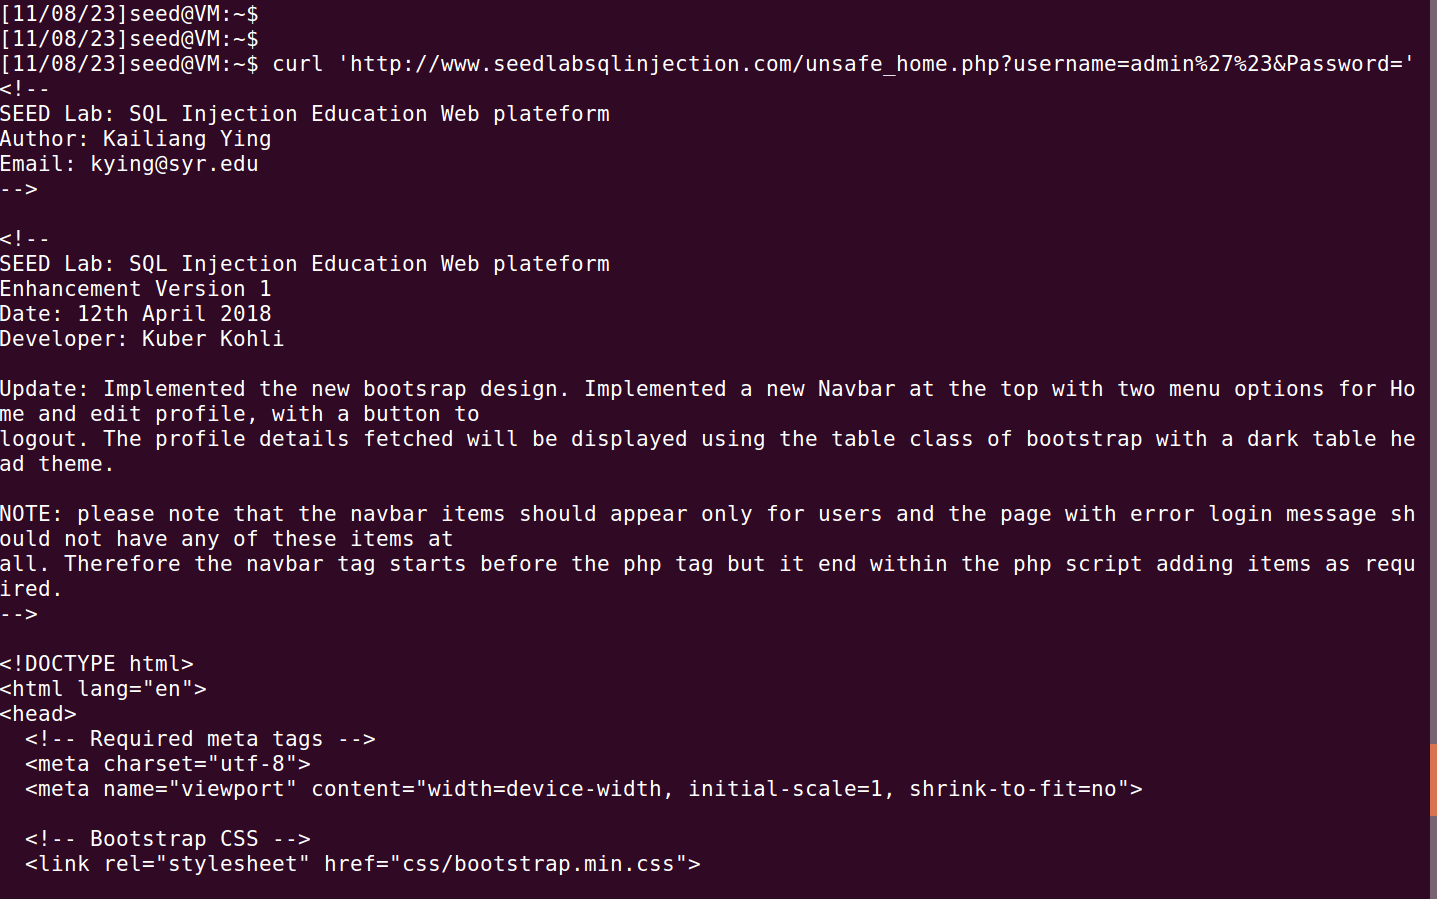
\includegraphics[scale=.34]{task2_2_1_sql.png}
    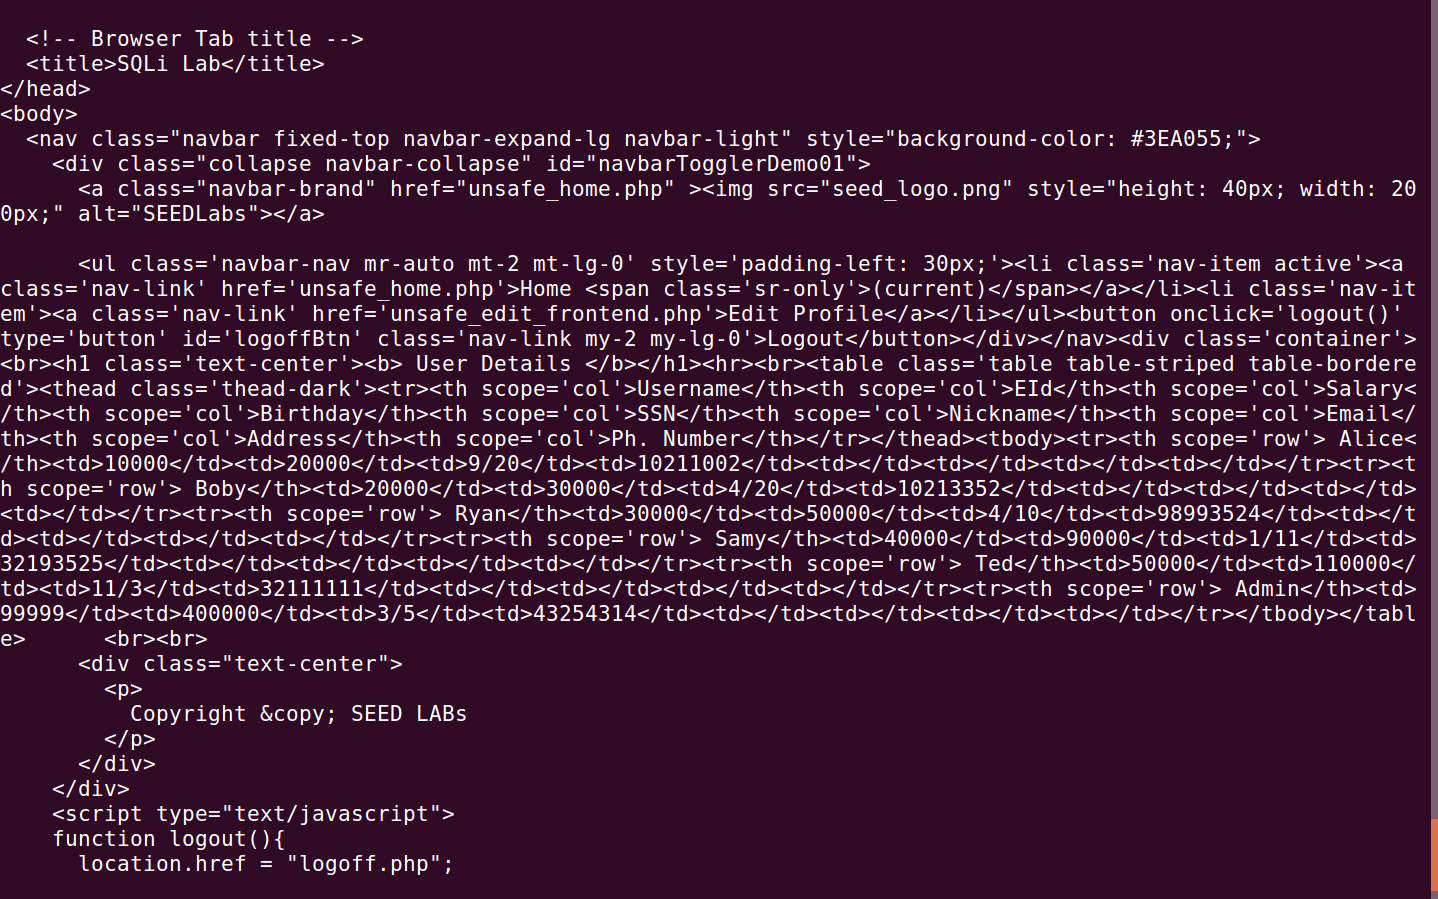
\includegraphics[scale=.34]{task2_2_2_sql.png}
\end{center}

Si bien a simple vista no se entiende mucho el contenido de la respuesta, copiandolo en un archivo y abriendolo en 
un navegador se renderiza la página con la información que se buscaba.

\subsubsection*{Task 2.3}
Luego de poder acceder a la información, queremos poder modificarla utilizando la misma vulnerabilidad. Esto se 
podría lograr con una segunda query. Se puede ingresar un usuario al autenticarse que haga justamente eso.
Un posible usuario es el siguiente: 

\verb|admin'; DELETE FROM credential WHERE Name = 'Alice'; #|

De esta manera, lograriamos autenticarnos como administrador y aparte se ejercutaría la segunda query que borra el 
registro del usuario \textit{Alice}. Se podría también hacer con una query UPDATE para modificar algún registro.

El inconveniente con el que nos encontramos, es que el método utilizado para ejercutar la query no soporta ejecución
multi-query, por lo que obtenemos un error del servidor al intentar loguearnos con el usuario antes mencionado y 
una constraseña cualquiera. El error fue el siguiente:
\begin{center}
    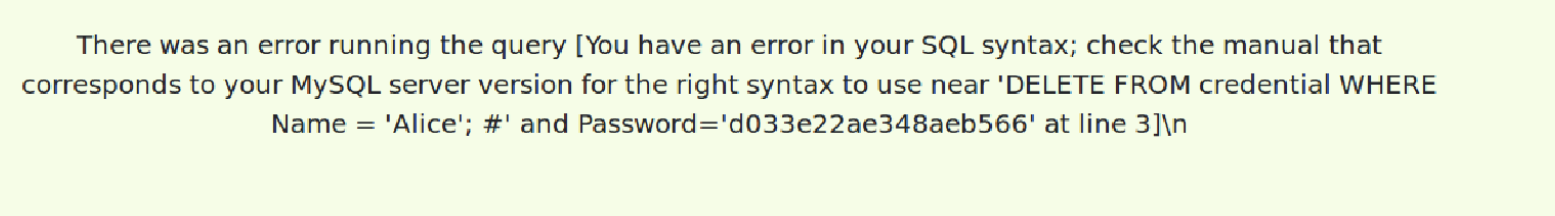
\includegraphics[scale=.45]{task2_3_sql.png}
\end{center}

Intentamos modificar el archivo .php donde se encuentra la implementación del login de la página web para utilizar 
otro método que si soporte ejecución multi-query, pero sin resultados positivos.

Para lograr alterar los datos de la base de datos se va a tener que explotar alguna otra vulnerabilidad, si la hay.

\subsection*{Task 3}
Se conoce otra vulnerabilidad de la aplicación, en este caso en la página que le permite a los empleados actualizar 
algunos de sus datos personales. Esta vulnerabilidad es similar a la anterior, pero con una declaración sql UPDATE,
lo cual es más peligroso ya que permite modificar los datos. Se puede tener acceso a esta página logueandose a un perfil
no administrador, usando la vulnerabilidad antes explotada.

\subsubsection*{Task 3.1}
Desde la página principal de la aplicación, nos logueamos al perfil de Alice, ingresando \verb|Alice'#| como usuario 
y sin la necesidad de conocer la contraseña. Estos son los datos actuales de su perfil:
\begin{center}
    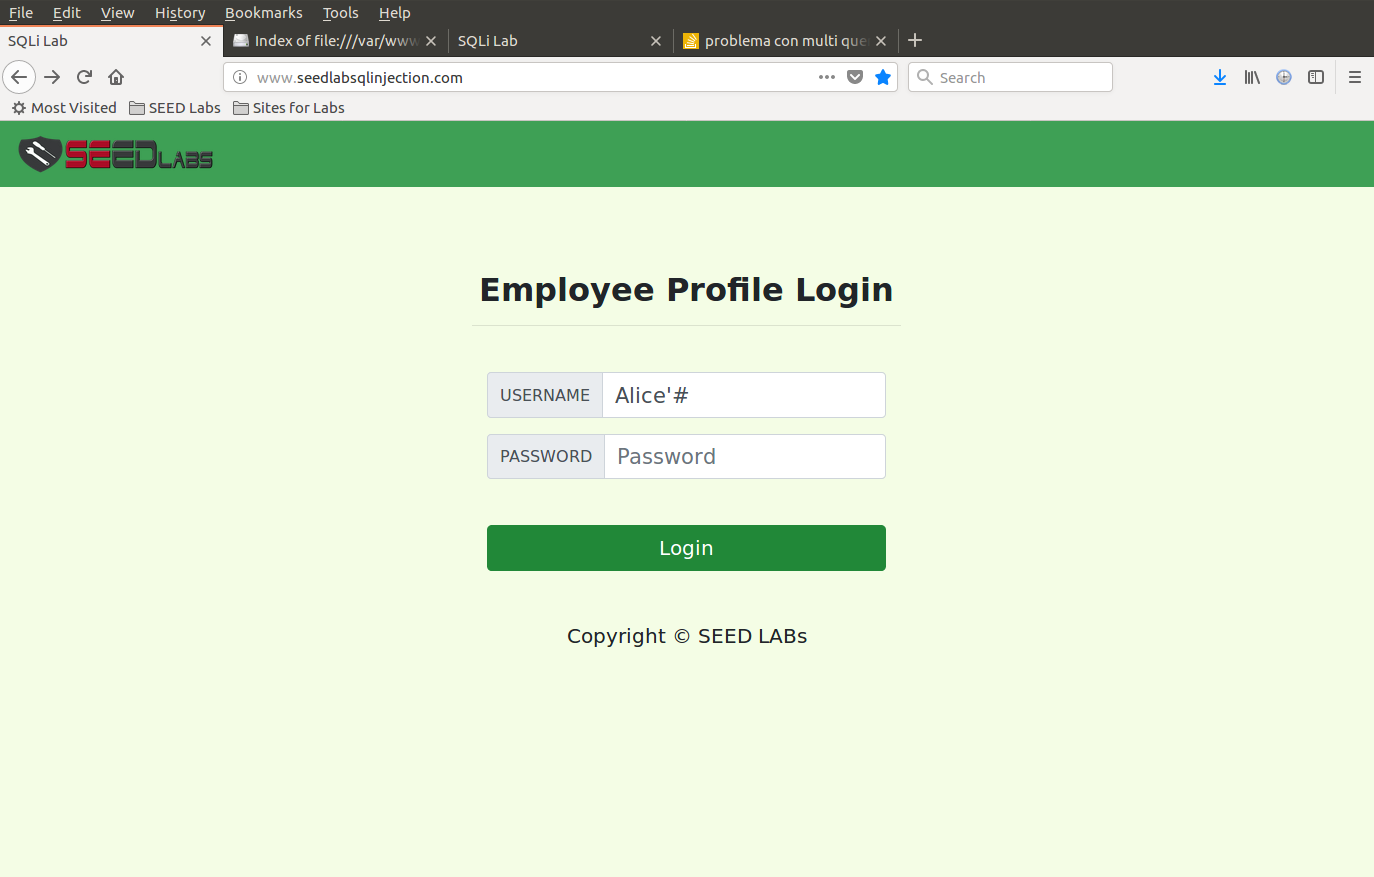
\includegraphics[scale=.35]{task3_1_1_sql.png}
    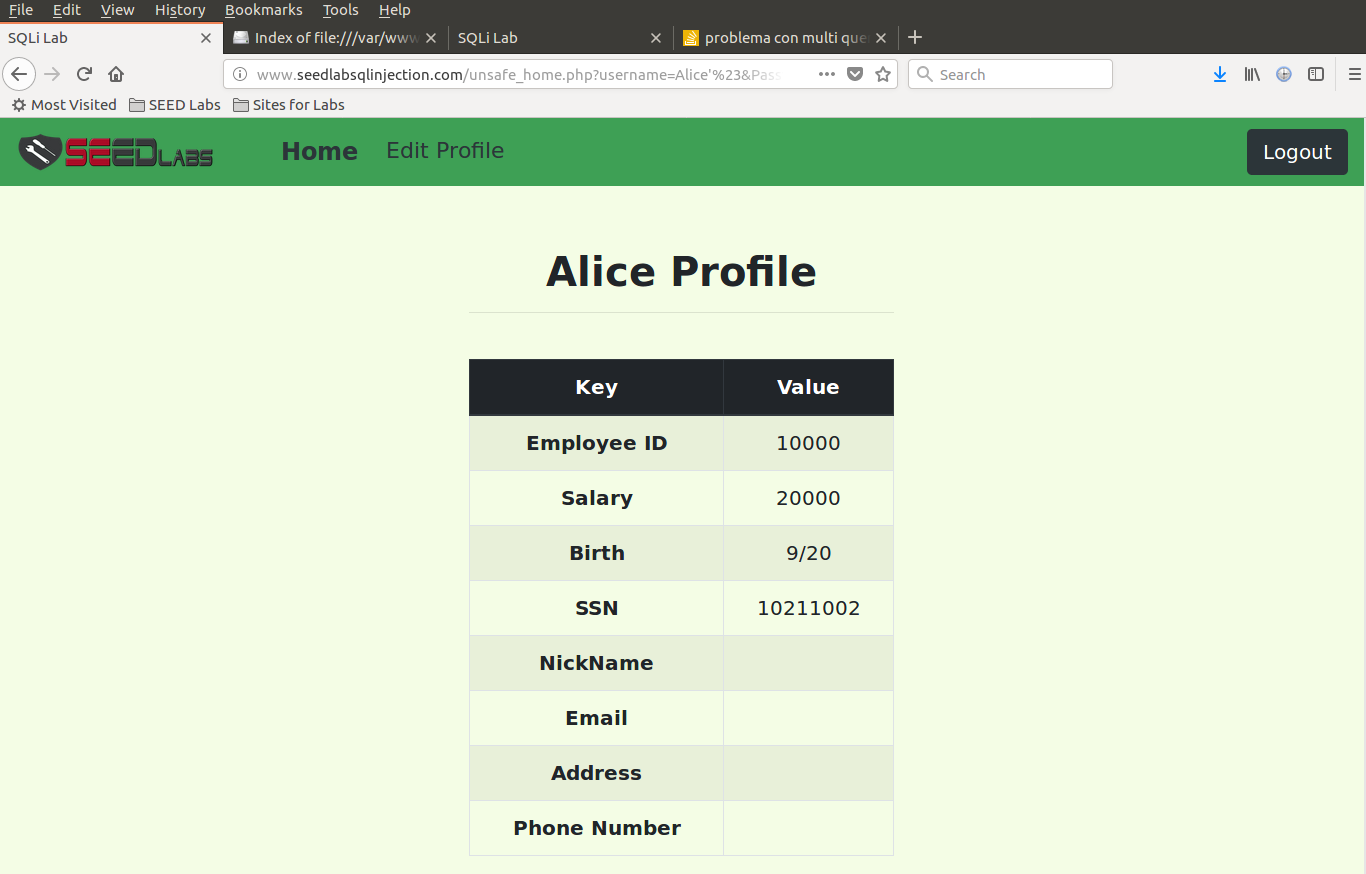
\includegraphics[scale=.35]{task3_1_2_sql.png}
\end{center}


Luego, queremos utilizar la página \verb|Edit Profile|, que permite editar algunos datos del perfil de Alice, 
para editar su salario, que  no es uno de los campos que se permiten editar. Para ellos, ingresamos lo siguiente 
en el campo de \verb|nickname|: \verb|Ali', salary = 100000 WHERE Name = 'Alice' #|. De esta manera el apodo 
de Alice pasara a ser Ali y su salario pasará a ser \$100000. A continuación, muestro como se ve esto desde la página:
\begin{center}
    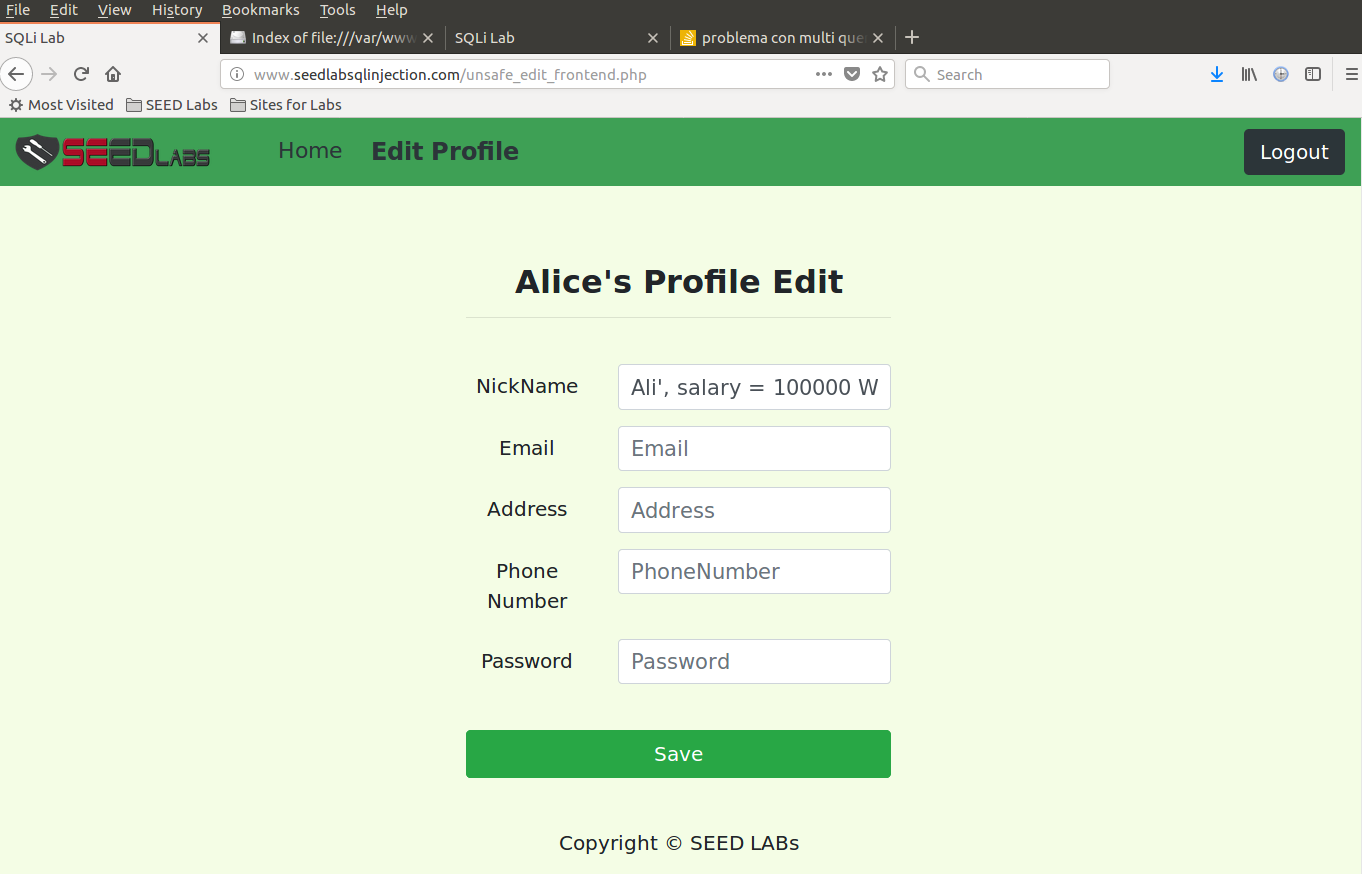
\includegraphics[scale=.34]{task3_1_3_sql.png}
    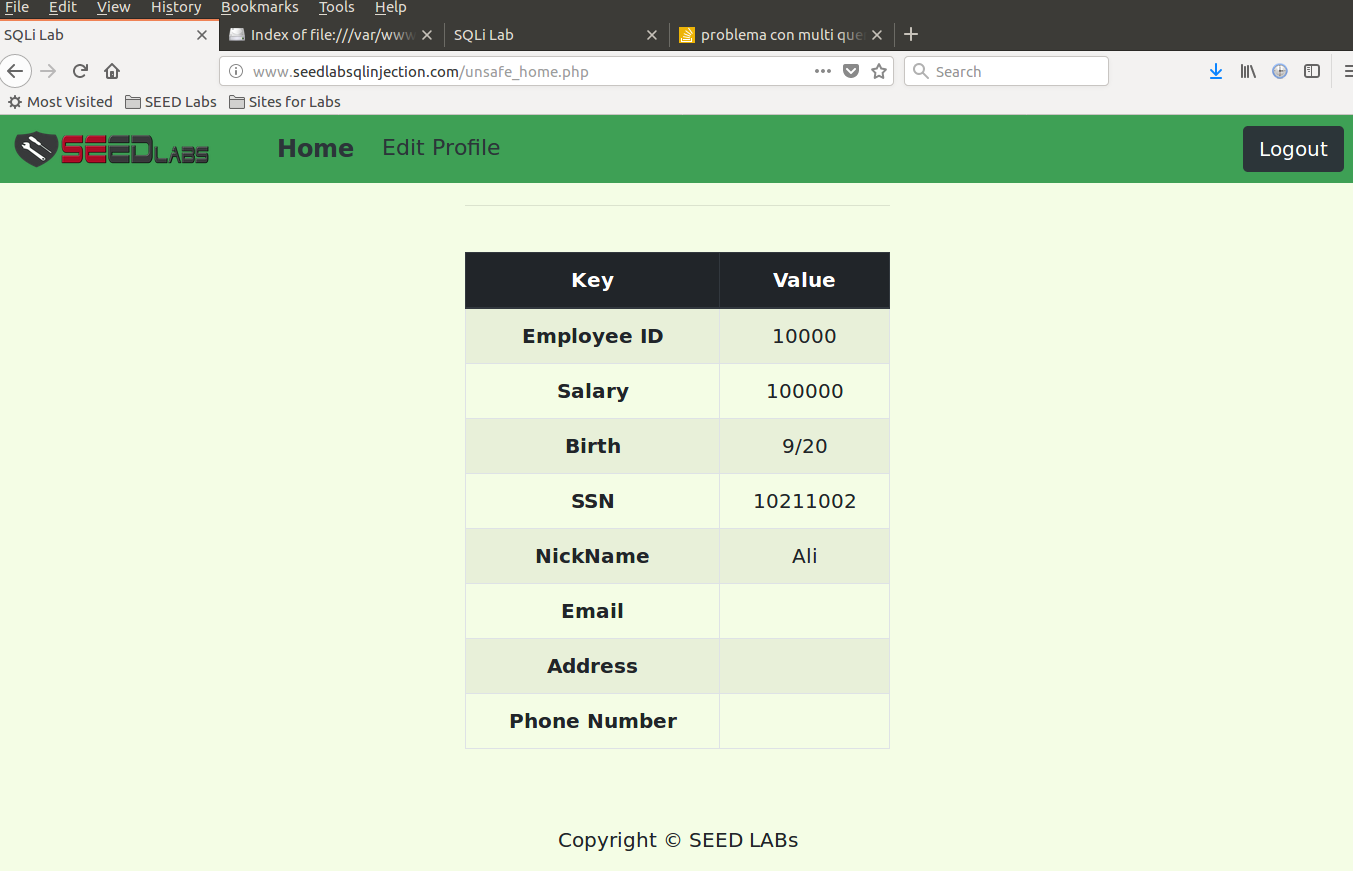
\includegraphics[scale=.34]{task3_1_4_sql.png}
\end{center}

\subsubsection*{Task 3.2}
La idea es ahora modificar el salario de Boby. Esto lo podemos lograr ingresando al perfil de Boby, o mismo 
desde el perfil de Alice en el que ya estamos logueados. Para hacerlo desde el perfil de Alice, nuevamente 
vamos a editar sus datos, pero esta vez ingresando \verb|', salary = 1 WHERE Name = 'Boby' #| en el campo 
\verb|nickname|. En lugar de definir un apodo como hicimos con Alice, directamente cerramos comillas y 
evitamos que el campo de apodo se modifique, para que no levante sospechas. A continuación muestro como se 
ven los datos de Boby previo a la modificación (el salario es 30000), como se ve la página donde hago la 
modificación, y finalmente como se ven los datos luego de ser modificados (el salario es 1):
\begin{center}
    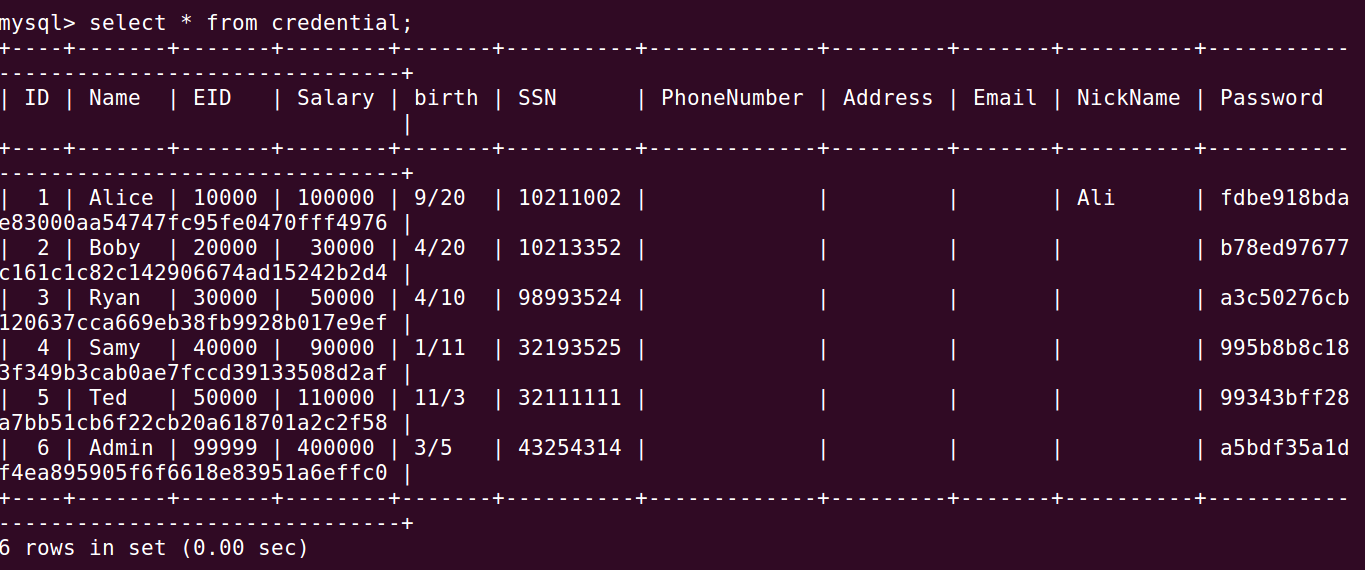
\includegraphics[scale=.34]{task3_2_1_sql.png}
    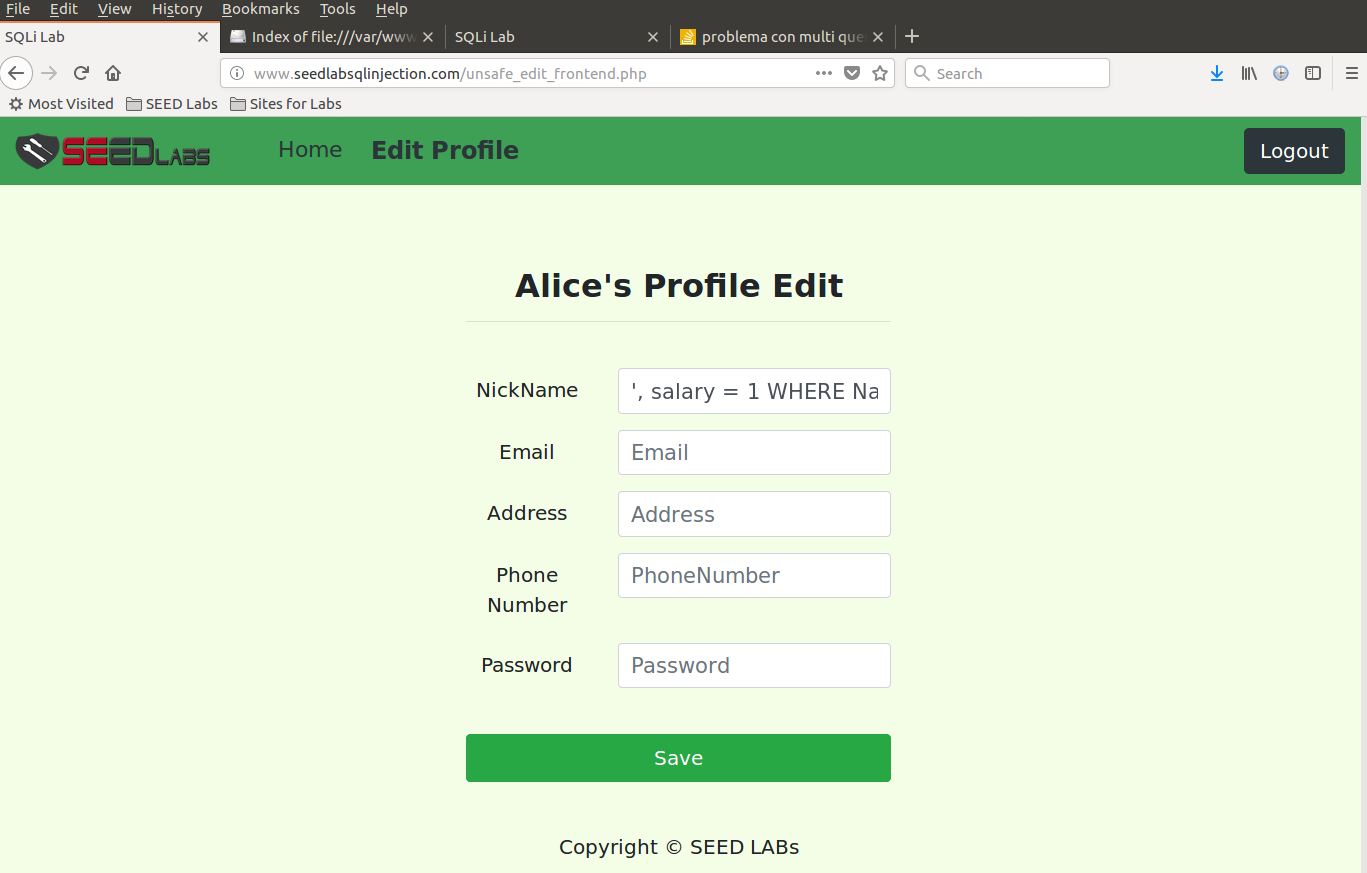
\includegraphics[scale=.34]{task3_2_2_sql.png}
    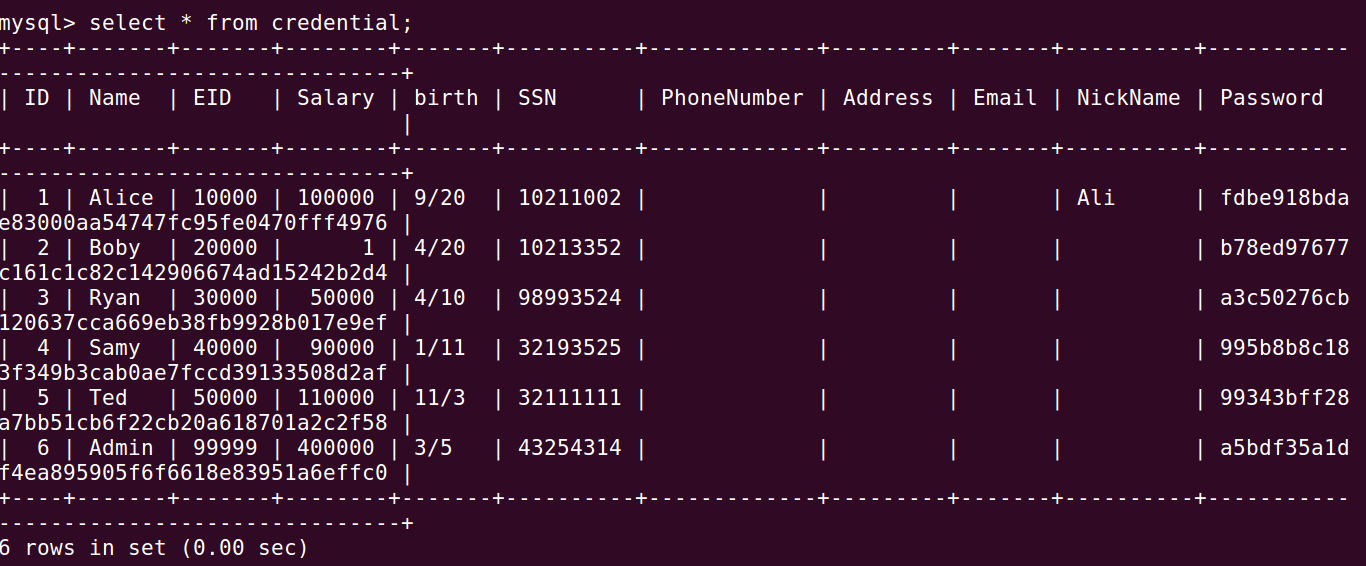
\includegraphics[scale=.34]{task3_2_3_sql.png}
\end{center}

\subsubsection*{Task 3.3}
Finalmente, se quiere modificar la contraseña de Boby. Nuevamente lo hacemos desde el perfil de Alice, en la página 
para editar datos personales. Para modificar la contraseña tenemos que tener algunas otras consideraciones, ya que 
las contraseñas no se guardan como texto plano en la base de datos, sino que se guarda el valor haseado con la 
función SHA1. En este caso, ingresamos en el campo \verb|nickname| lo siguiente: \\
\verb|', Password = sha1(password) WHERE Name = 'Boby' #|. De vuelta, no se modifica el valor del apodo y la función 
\verb|sha1| es la que se le aplica a la contraseña para guardar el valor hasheado.
De la imagen inmediata anterior donde se muestran los datos de la tabla luego de modificar el salario de Boby, vemos
que el hash de la contraseña de Boby comienza con \verb|b78...|.
Realizamos la modificación, y nuevamente visualizamos los datos de la tabla:
\begin{center}
    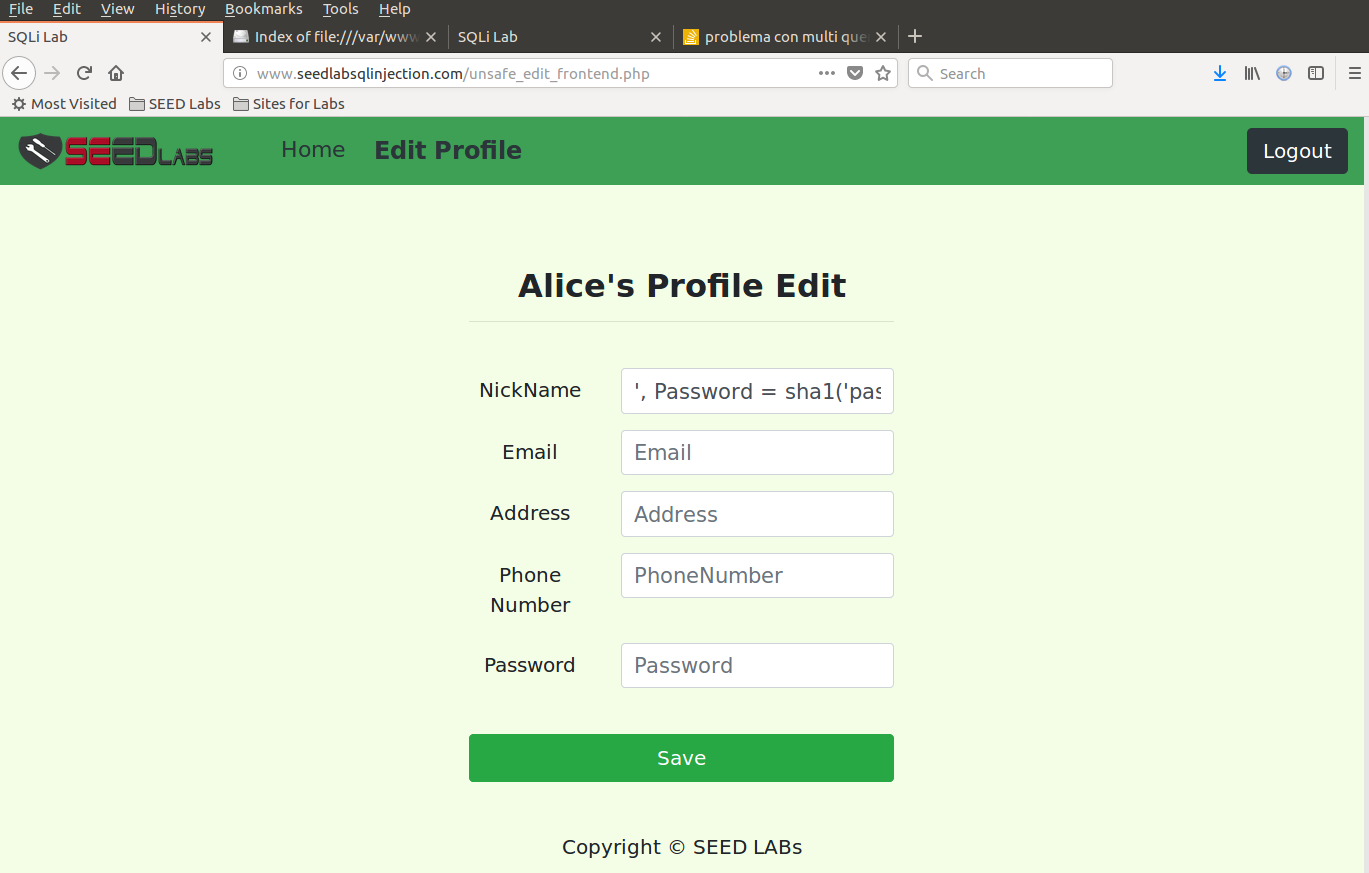
\includegraphics[scale=.34]{task3_3_1_sql.png}
    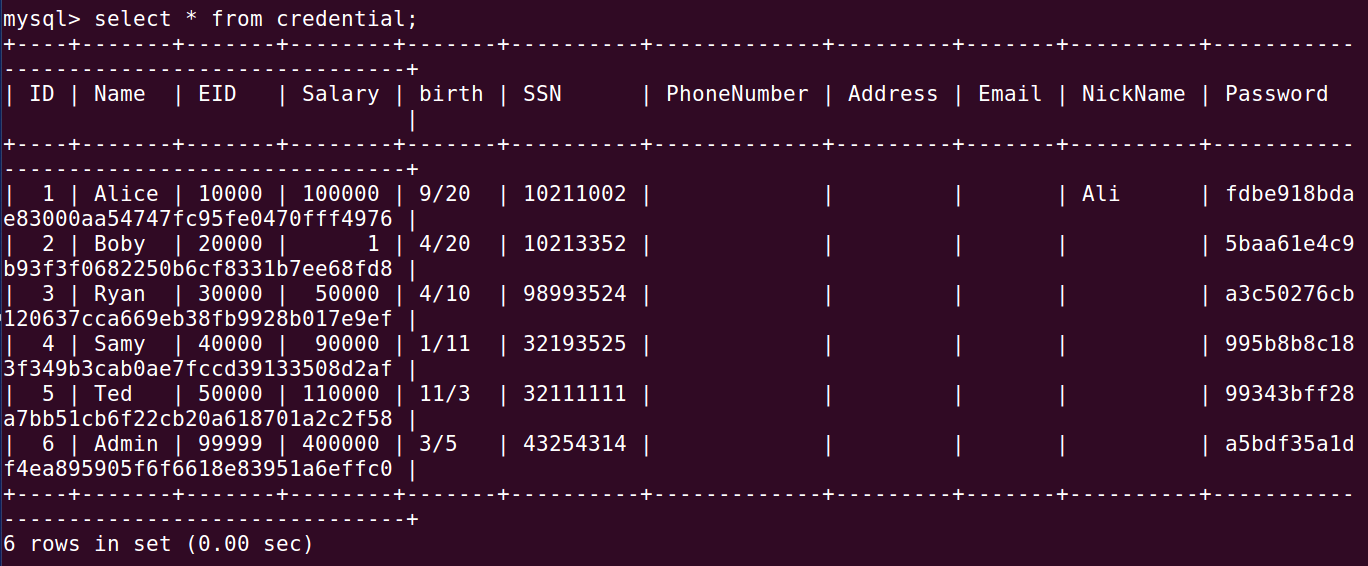
\includegraphics[scale=.34]{task3_3_2_sql.png}
\end{center}

Notese que el hash de la contraseña de Boby comienza con \verb|5ba...|, con lo cual comprobamos que fue modificada.
Probamos ingresar al perfil de Boby con la nueva contraseña, y lo conseguimos:
\begin{center}
    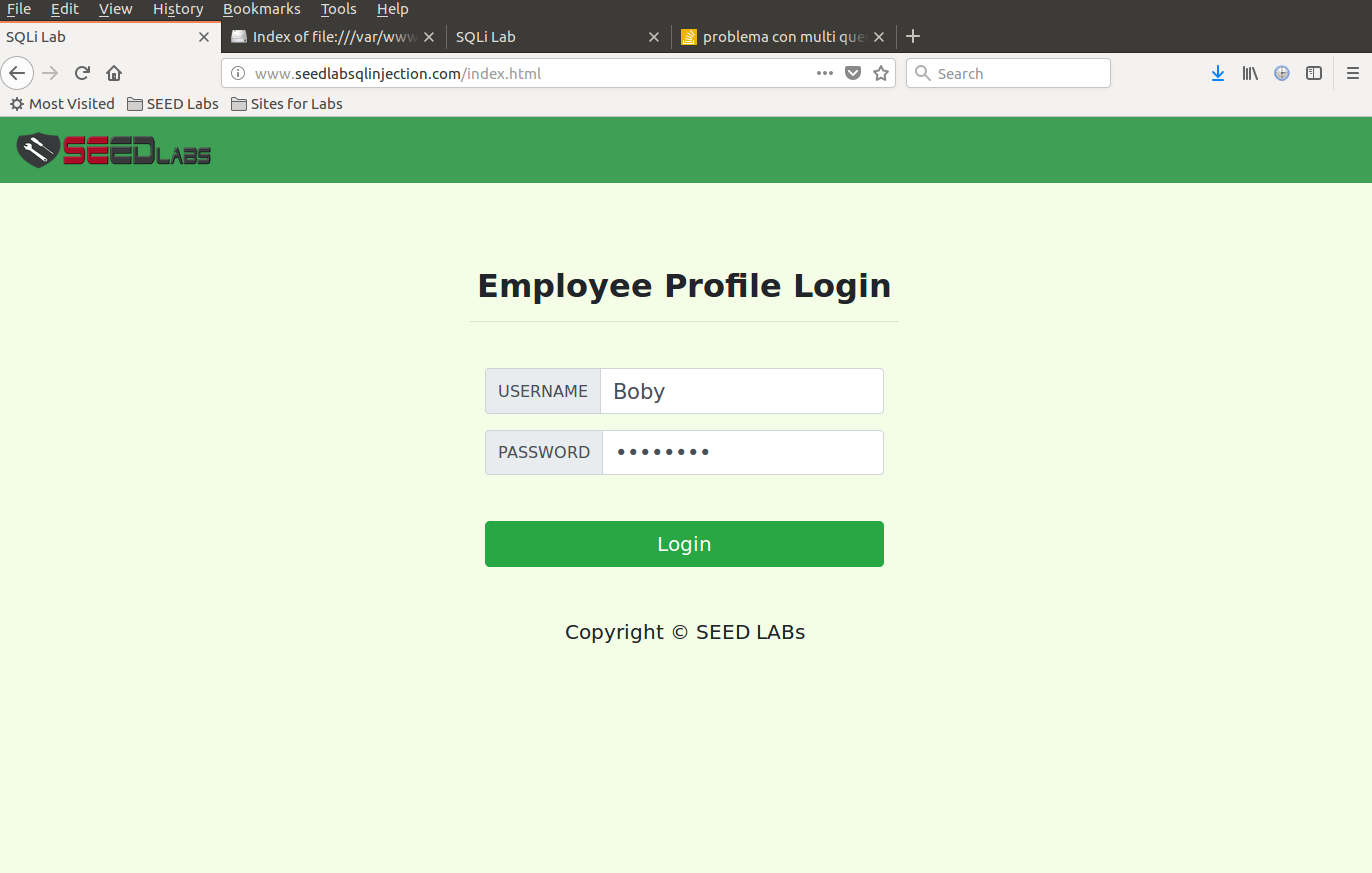
\includegraphics[scale=.34]{task3_3_3_sql.png}
    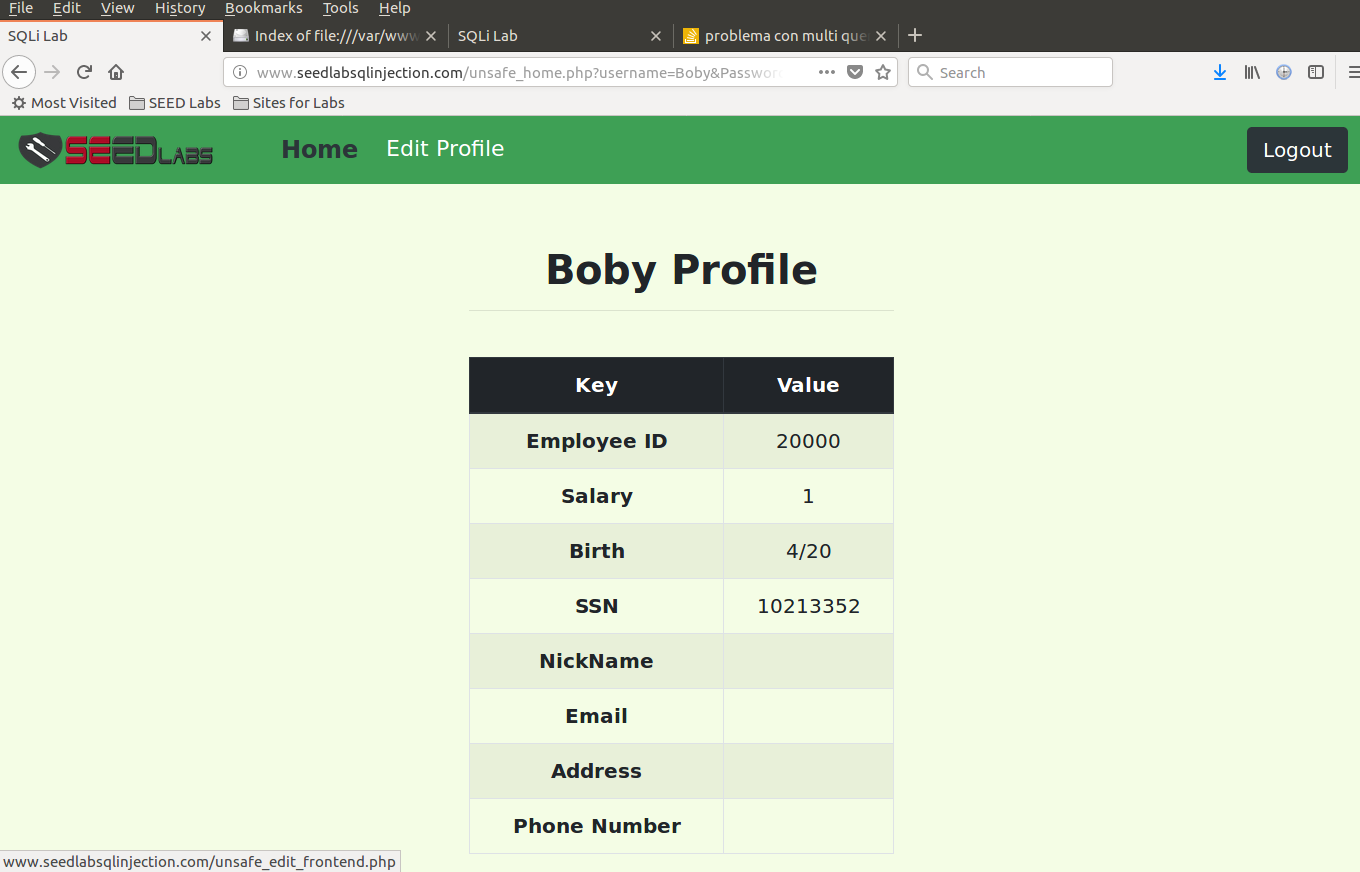
\includegraphics[scale=.34]{task3_3_4_sql.png}
\end{center}


\section*{Criptografía}
Tema realizado en modo básico.

\subsection*{Ejercicio 2}
\textit{Data Encryption Standard}, también conocido como DES, es de los primeros cifradores simétricos de bloque.
El cifrador DES utiliza claves de 56 bits, es por eso que en la actualidad es considerado inseguro y ya no se 
utiliza, al menos no en su versión básica. Una alternativa podría ser tener dos claves, $k_1$ y $k_2$, y encriptar 
el mensaje usando primero $k_1$, y luego encriptar el resultado usando $k_2$. Llamemos este nuevo cifrador DES2, 
y siendo $DES_e$ un cifrador de DES y $t$ el mensaje a encriptar, entonces la encriptación 
de DES2 sería la siguiente:
$$DES2(t,k_1,k_2) = DES_e(DES_e(t,k_1),k_2)$$
Luego, siendo $DES_d$ un descifrador de DES y $t$ el mensaje a desencritar, la desencriptación consistiría en:
$$DES2(t,k_1,k_2) = DES_d(DES_d(t,k_2),k_1)$$

La vulnerabilidad que volvió obsoleto al cifrador DES no es propia del algoritmo de cifrado, sino que fueron los 
ataques por fuerza bruta. Con el avance de la capacidad de cómputo, estos ataques se volvieron muy rápidos por la 
corta longitud de las claves que utiliza, acortando la vida útil de las claves DES hasta volverlas inutilizables. 
En este sentido, el cifrado doble que se propone sufre la misma vulnerabilidad. Si bien pareciera ser más efectivo
que un cifrado DES simple, y aunque puede ofrecer mayor resistencia a un ataque por busqueda exhaustiva ya que 
requerirá de más tiempo y memoria, no ofrece mayor seguridad.
siempre suponiendo que la elección de las claves es realmente aleatoria

\subsection*{Ejercicio 6}
El cifrador DES encripta bloques de 64 bits. Es por esto que existen distintos \textit{modos de operación} para 
poder encriptar textos de longitud arbitraria. Dos de los modos de operación son \textit{Electronic Code Book} (ECB) 
y \textit{Cipher Block Chaining} (CBC).

ECB consiste en dividir el texto legible en bloques de 64 bits, cada bloque se encripta con una misma clave y 
el resultado es el texto obtenido de concatenar todos los bloques de 64 bits de texto cifrado. El proceso de 
desencriptación es análogo. Este modo de operación implica que de bloques legibles iguales se obtengas bloques 
cifrados iguales, ya que el cifrado de cada bloque es independiente del resto.

CBC, por su parte, es un poco más complejo. También se divide el texto legible en bloques de 64, y se elige un 
vector de inicialización. Se hace una operación XOR entre el vector de inicialización y el primer bloque de texto
legible, y el resultado se encripta con la clave. Luego se hace una operación XOR entre el texto cifrado del primer
bloque y el texto legible del segundo, y devuelta el resultado se encripta con la clave, y así sucesivamente hasta
encriptar el último bloque. El resultado final consiste de la concatenación de todos los bloques cifrados intermedios.
Con este modo de operación se logra que bloques iguales de texto legible no resulten en bloques iguales de texto 
cifrado, ya que el cifrado de cada bloque depende de todos los bloques anteriores.

Para encriptar el contenido de una imagen representada en un mapa de bits recomendaría el modo CBC, ya que en una 
imagen es muy alta la probabilidad de encontrar bloques de bits iguales, y un cifrado ECB revelaría este patrón en 
el texto cifrado, potencialmente simplificando un ataque.




\end{document}